% CVPR 2026 Paper Template; see https://github.com/cvpr-org/author-kit

\documentclass[10pt,twocolumn,letterpaper]{article}

%%%%%%%%% PAPER TYPE  - PLEASE UPDATE FOR FINAL VERSION
\usepackage{cvpr}              % To produce the CAMERA-READY version
% \usepackage[review]{cvpr}      % To produce the REVIEW version
% \usepackage[pagenumbers]{cvpr} % To force page numbers, e.g. for an arXiv version

% Import additional packages in the preamble file, before hyperref
\input{preamble}

% It is strongly recommended to use hyperref, especially for the review version.
% hyperref with option pagebackref eases the reviewers' job.
% Please disable hyperref *only* if you encounter grave issues, 
% e.g. with the file validation for the camera-ready version.
%
% If you comment hyperref and then uncomment it, you should delete *.aux before re-running LaTeX.
% (Or just hit 'q' on the first LaTeX run, let it finish, and you should be clear).
\definecolor{cvprblue}{rgb}{0.21,0.49,0.74}
\usepackage[pagebackref,breaklinks,colorlinks,allcolors=cvprblue]{hyperref}

% Use the postscript times font!
\usepackage{lipsum} 
\usepackage{times}
\usepackage{soul}
\usepackage{url}
\usepackage{amsthm}
\usepackage{booktabs}
\usepackage{algorithm}
\usepackage{algorithmic}
\usepackage[switch]{lineno}
\usepackage{color, colortbl}
\usepackage{comment}
\usepackage{xcolor}
\usepackage{tabularx}
% \usepackage{todonotes}
\usepackage{kotex}
\usepackage{multirow}
\usepackage{appendix}
\usepackage{makecell}
\usepackage{tcolorbox}
\usepackage{tikz}
\usepackage{pgfplots}
\pgfplotsset{compat=1.17}

% Define promptbox environment
\newtcolorbox{promptbox}[1][]{
    colback=gray!5!white,
    colframe=gray!75!black,
    fonttitle=\bfseries\small,
    title=#1,
    boxrule=0.5pt,
    arc=2pt,
    left=6pt,
    right=6pt,
    top=4pt,
    bottom=4pt
}

\newcommand{\lsp}[1]{\todo[inline,color=blue!20!white]{\textbf{Seungpil:} #1}}
\newcommand{\kdy}[1]{\todo[inline,color=green!20!white]{\textbf{Daeyeon:} #1}}

%%%%%%%%% PAPER ID  - PLEASE UPDATE
\def\paperID{*****} % *** Enter the Paper ID here
\def\confName{CVPR}
\def\confYear{2026}

%%%%%%%%% TITLE - PLEASE UPDATE
\title{Enhancing 3D Spatial Reasoning in Vision-Language Models through Multi-View Augmentation and Quaternion-Based Representation}

%%%%%%%%% AUTHORS - PLEASE UPDATE
\author{Seungpil Lee\\
Gwangju Institute of Science and Technology \\
% Institution1 address\\
{\tt\small iamseungpil@gm.gist.ac.kr}
% For a paper whose authors are all at the same institution,
% omit the following lines up until the closing ``}''.
% Additional authors and addresses can be added with ``\and'',
% just like the second author.
% To save space, use either the email address or home page, not both
\and
Daeyeon Kim\\
Gwangju Institute of Science and Technology\\
% First line of institution2 address\\
{\tt\small daeyeonkim@gm.gist.ac.kr}
}

\begin{document}
\maketitle

\begin{abstract}
Spatial reasoning in vision-language models is constrained by the fundamental ambiguity of single-view observations: depth ordering, scale-distance relationships, and relative positions often cannot be reliably inferred from a single image. We address this limitation through multi-view reasoning, synthesizing complementary viewpoints via generative models and training vision-language models to integrate information across views. Our approach employs MVGenMaster for photorealistic view synthesis and introduces view-aware chain-of-thought supervision with coordinate transformation to ensure geometric consistency. Critically, we demonstrate that multi-view training benefits are realized only when inference follows the same dual-view paradigm---models trained on multi-view data but tested on single images fail to improve. With aligned training and inference, our method achieves 60.1\% accuracy on 3DSRBench, comparable to SpatialReasoner (60.3\%) which relies on reinforcement learning, while providing an alternative framework based on geometric consistency across synthesized viewpoints. Code is available at \url{https://github.com/Multiview-geometry-gist/SpatialReasoner}.
\end{abstract}

\section{Introduction}
\label{sec:intro}
Spatial reasoning from visual observations is fundamental for intelligent systems interacting with physical environments. Vision-language models have achieved remarkable progress in understanding 3D spatial relationships from images, enabling applications in robotic manipulation~\cite{bohg2014robot}, augmented reality~\cite{azuma1997survey}, and autonomous navigation~\cite{boninfont2008visual}. Recent approaches extract metric spatial information using monocular depth estimation~\cite{yang2024depth} and scene understanding~\cite{ravi2024sam} to ground natural language queries about object positions, distances, and orientations.

Despite this progress, single-view spatial reasoning faces an intrinsic limitation: the projection from 3D to 2D is inherently lossy. Depth ordering becomes ambiguous when objects lack strong monocular cues, scale and distance trade off in producing identical image appearances, and occlusions hide spatial relationships. Methods such as SpatialVLM~\cite{chen2024spatialvlm}, SpatialRGPT~\cite{cheng2024spatialrgpt}, and SpatialReasoner~\cite{ma2025spatialreasoner} address this through increasingly sophisticated reasoning pipelines, yet remain fundamentally constrained by the information available in a single view.

We approach spatial reasoning from a multi-view perspective, leveraging the geometric constraint that consistent 3D structure must explain observations from multiple viewpoints. Novel views are synthesized using MVGenMaster~\cite{ren2025mvgenmaster}, a generative model that produces photorealistic images without the artifacts of geometric projection methods. The model is trained on paired views with view-aware chain-of-thought supervision, learning to integrate complementary geometric information for spatial inference.

A key finding of our work is that multi-view training confers benefits only when inference maintains the same paradigm. Models trained on synthesized multi-view data but evaluated on single images fail to outperform simpler baselines, revealing a distribution mismatch between training and testing conditions. When both training and inference utilize dual-view inputs, our approach achieves 60.1\% accuracy on 3DSRBench, demonstrating that multi-view consistency provides a viable path toward robust spatial understanding.

This work makes three contributions. First, we propose a multi-view spatial reasoning framework as an alternative to reinforcement learning approaches. While SpatialReasoner~\cite{ma2025spatialreasoner} achieves state-of-the-art performance through chain-of-thought supervision followed by GRPO-based refinement, our approach instead leverages geometric consistency across synthesized viewpoints, achieving comparable accuracy without reinforcement learning. Second, we introduce view-aware chain-of-thought supervision with coordinate transformation, ensuring that spatial descriptions remain consistent with each synthesized viewpoint. Third, we provide empirical analysis demonstrating the necessity of train-test alignment for realizing multi-view benefits---models trained on multi-view data but evaluated on single images fail to improve, an insight with implications for future multi-view learning approaches.

\begin{figure*}[ht!]
\centering
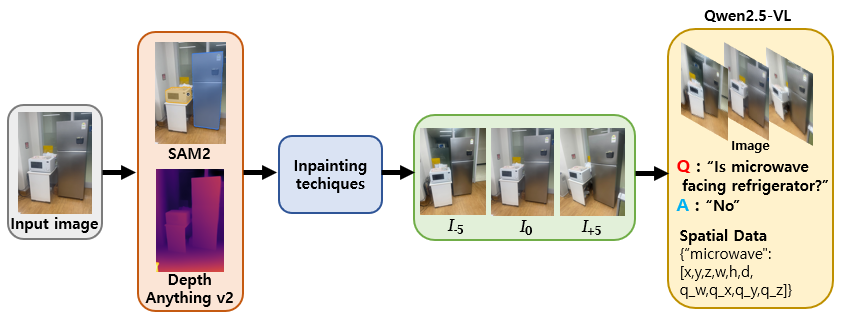
\includegraphics[width=0.8\textwidth]{figures/dummy.png}
\caption{Overview of multi-view spatial reasoning pipeline. Given an input image, MVGenMaster synthesizes a rotated view at $10^\circ$ azimuth. Both views are presented to the model with explicit viewpoint annotations. Chain-of-thought supervision incorporates coordinate transformation to ensure spatial descriptions remain consistent with each view's perspective. During inference, the same dual-view paradigm is maintained for train-test alignment.}
\label{fig:view-synthesis-overview}
\end{figure*}

% \section{Related Work}
\label{sec:related}

\subsection{Spatial Reasoning in Vision-Language Models}

Recent vision-language models have made significant progress in understanding spatial relationships within images. SpatialVLM~\cite{chen2024spatialvlm} introduced large-scale synthetic data generation for training models on spatial reasoning tasks, demonstrating improved performance on distance estimation and directional queries. SpatialRGPT~\cite{cheng2024spatialrgpt} enhanced spatial understanding through region-aware representations and depth integration, enabling more precise reasoning about object relationships. Most recently, SpatialReasoner~\cite{ma2025spatialreasoner} proposed explicit 3D representations to bridge perception and reasoning stages. However, these approaches fundamentally rely on single-view observations, which inherently suffer from depth ambiguity and scale uncertainty. Single-view depth estimation models~\cite{yang2024depth} provide relative depth but cannot resolve metric scale without additional constraints. Furthermore, existing methods typically represent object orientation using Euler angles~\cite{chen2024spatialvlm,ma2025spatialreasoner}, which exhibit discontinuities at gimbal lock configurations and complicate rotation-based reasoning tasks. These limitations motivate our approach of leveraging multi-view geometric consistency during training while maintaining single-image inference.

\subsection{Geometric Representations for 3D Understanding}

Multi-view geometry has long been recognized as essential for robust 3D reconstruction and understanding~\cite{hartley2003multiple}. Traditional structure-from-motion pipelines exploit multi-view consistency to resolve depth ambiguities and estimate metric scale. Recent work has explored incorporating multi-view information into learning-based approaches, though typically requiring multiple images at inference time. Our method differs by synthesizing geometrically consistent views from estimated depth maps~\cite{yang2024depth} during training only, allowing the model to learn implicit multi-view reasoning without additional inference cost. For rotation representation, computer graphics and robotics communities have established quaternions as the preferred parameterization due to their mathematical properties~\cite{shoemake1985animating}. Quaternions provide singularity-free representation, enable smooth interpolation through spherical linear interpolation, and naturally support composition operations. Despite these advantages, vision-language models have predominantly used Euler angles or rotation matrices for pose representation. We adopt unit quaternions for object orientation, enabling more stable gradient flow during training and more reliable rotation-based spatial reasoning at inference time.

\section{Method}
\label{sec:methods}

\subsection{Overview}

Multi-view consistency provides a fundamental constraint for 3D spatial understanding. Our approach leverages this principle by training vision-language models to reason about spatial relationships from multiple synthesized viewpoints. Unlike depth-based methods that suffer from occlusion artifacts and require complex inpainting, we employ a generative view synthesis model that produces photorealistic novel views while preserving scene semantics. The training pipeline integrates these synthesized views with viewpoint-aware chain-of-thought supervision, enabling the model to learn to integrate spatial information across multiple views.

\subsection{Generative View Synthesis}

High-fidelity view synthesis is essential for multi-view spatial reasoning. We adopt MVGenMaster~\cite{ren2025mvgenmaster}, a video diffusion model that generates temporally coherent novel views from a single input image. Given an input image $I_0$, the model synthesizes a rotated view $I_\theta$ by conditioning on the desired camera transformation:
\begin{equation}
I_\theta = \mathcal{G}(I_0, \Delta\phi, \Delta\theta)
\end{equation}
where $\Delta\phi$ and $\Delta\theta$ represent azimuth and elevation changes respectively. The diffusion-based generation produces complete images with reduced artifacts compared to geometric projection methods that require occlusion handling and hole-filling.

We generate views at $\pm 10^\circ$ azimuth rotation, balancing viewpoint diversity with semantic preservation. This small rotation angle ensures that spatial relationships remain interpretable while providing sufficient geometric variation for robust 3D understanding. Each training sample thus consists of paired views $(I_0, I_{10^\circ})$ depicting the same scene from complementary perspectives.

\subsection{View-Aware Chain-of-Thought Transformation}

Spatial reasoning benefits from explicit geometric reasoning in chain-of-thought format. However, standard chain-of-thought annotations describe spatial relationships from a fixed viewpoint, creating inconsistency when paired with rotated views. We address this through coordinate transformation that adapts spatial descriptions to each viewpoint.

For an object at position $(x, y, z)$ in the original view, its coordinates in a rotated view are computed via:
\begin{equation}
\begin{bmatrix} x' \\ y' \\ z' \end{bmatrix} = R_\theta \begin{bmatrix} x \\ y \\ z \end{bmatrix}
\end{equation}
where $R_\theta$ is the rotation matrix corresponding to camera transformation. Directional relationships (left/right, front/back) are similarly transformed to maintain consistency with the visual content. This view-aware transformation enables the model to learn that spatial relationships are observer-dependent while the underlying 3D structure remains invariant.

\subsection{Multi-View Training Framework}

The training objective encourages view-consistent spatial understanding. For each sample, we construct multi-view inputs by concatenating the original and synthesized views with explicit viewpoint annotations, specifying the rotation angle for each view before presenting the spatial reasoning question. This structured format enables the model to associate each visual input with its corresponding viewpoint, facilitating cross-view reasoning. The prompt template is illustrated below.

\begin{promptbox}[Multi-View Spatial Reasoning Prompt]
\small
View 1 (rotation: 0 degrees):\\
View 2 (rotation: 10 degrees):\\
\\
Question: Is the cup to the left of the bottle?\\
Options:\\
A. Yes \quad B. No\\
\\
Let's think step by step.\\
The cup is at position (0.3, 0.5, 2.1).\\
The bottle is at position (0.7, 0.4, 2.3).\\
Comparing x-coordinates: 0.3 < 0.7.\\
Therefore, the cup is to the left of the bottle.\\
Answer: A
\end{promptbox}

We fine-tune Qwen2.5-VL~\cite{bai2025qwen25vl} using LoRA~\cite{hu2021lora} on the augmented dataset. The model processes both views jointly, learning to integrate information across viewpoints for spatial inference. Chain-of-thought supervision with view-transformed coordinates provides intermediate reasoning steps, guiding the model toward geometrically grounded predictions.

\subsection{Multi-View Inference}

Inference follows the same multi-view paradigm established during training. Given a test image, we synthesize an additional view at $10^\circ$ rotation and present both views to the model with consistent formatting. This approach maintains the train-test alignment crucial for multi-view reasoning, allowing the model to leverage complementary geometric information from both viewpoints. The dual-view input provides parallax cues that disambiguate depth relationships otherwise challenging to infer from a single image.

\section{Experiments}
\label{sec:experiments}

\subsection{Experimental Setup}

We evaluate our approach on 3DSRBench~\cite{ma2025spatialreasoner}, a comprehensive benchmark for 3D spatial reasoning containing 11,686 questions across diverse spatial relationship categories. The benchmark covers distance estimation, directional reasoning, size comparison, and complex spatial queries requiring multi-step inference. All models use Qwen2.5-VL-7B-Instruct~\cite{bai2025qwen25vl} as the base architecture, fine-tuned with LoRA (rank 256) using the same hyperparameters for fair comparison.

View synthesis is performed using MVGenMaster, which generates video sequences depicting camera motion around the scene. We extract the final frame corresponding to the target rotation angle. For the full benchmark, we pre-generate $10^\circ$ rotated views for all 3,587 unique images, ensuring consistent view quality across evaluation runs.

\subsection{Quantitative Analysis}

Table~\ref{tab:main-results} and Figure~\ref{fig:accuracy-comparison} present the main experimental results comparing our multi-view approach against baseline methods.

\begin{table}[ht]
\centering
\begin{tabular}{lc}
\toprule
\textbf{Model} & \textbf{Accuracy (\%)} \\
\midrule
\multicolumn{2}{l}{\textit{Proprietary Models}} \\
GPT-4o~\cite{openai2024gpt4o} & 44.2 \\
Gemini 2.0~\cite{google2024gemini} & 51.1 \\
Qwen2.5-VL-Max~\cite{bai2025qwen25vl} & 52.0 \\
\midrule
\multicolumn{2}{l}{\textit{Open-Source Models}} \\
Qwen2.5-VL-7B & 48.3 \\
SpatialReasoner-SFT~\cite{ma2025spatialreasoner} & 58.3 \\
SpatialReasoner~\cite{ma2025spatialreasoner} & 60.3 \\
\midrule
\multicolumn{2}{l}{\textit{Our Approach}} \\
+ SFT (reproduced) & 58.0 \\
+ SFT + Mixed Aug & 60.2 \\
+ MVGen Multi-View & 60.1 \\
\bottomrule
\end{tabular}
\caption{Accuracy on 3DSRBench. Results for proprietary and SpatialReasoner models are from~\cite{ma2025spatialreasoner}. Our multi-view approach achieves comparable performance to SpatialReasoner while using a different methodology based on synthesized view pairs.}
\label{tab:main-results}
\end{table}

\begin{figure}[ht]
\centering
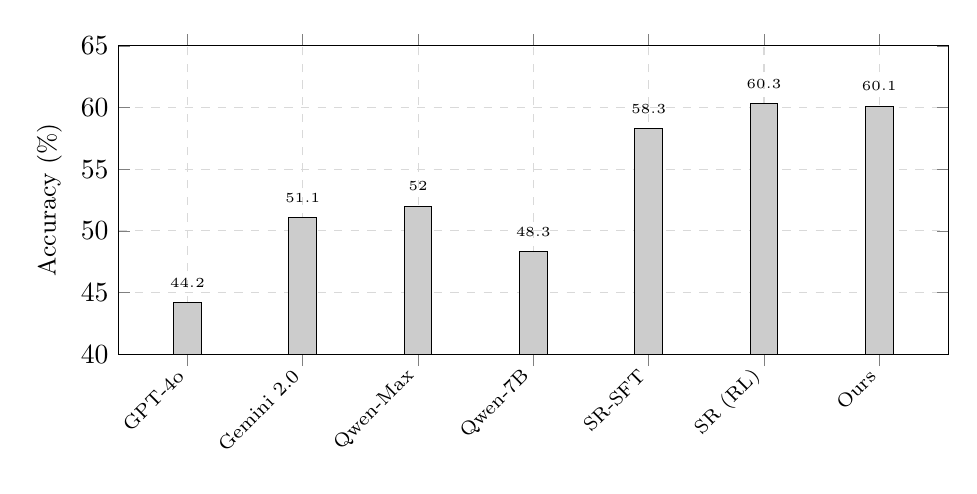
\begin{tikzpicture}
\begin{axis}[
    ybar,
    width=\columnwidth,
    height=5.5cm,
    ylabel={Accuracy (\%)},
    ylabel style={font=\small},
    ymin=40,
    ymax=65,
    ytick={40,45,50,55,60,65},
    xtick=data,
    symbolic x coords={GPT-4o, Gemini 2.0, Qwen-Max, Qwen-7B, SR-SFT, SR (RL), Ours},
    x tick label style={rotate=45, anchor=east, font=\scriptsize},
    bar width=10pt,
    nodes near coords,
    nodes near coords style={font=\tiny},
    every node near coord/.append style={yshift=2pt},
    enlarge x limits=0.1,
    grid=major,
    grid style={dashed, gray!30},
]
\addplot[fill=gray!40] coordinates {(GPT-4o, 44.2) (Gemini 2.0, 51.1) (Qwen-Max, 52.0) (Qwen-7B, 48.3) (SR-SFT, 58.3) (SR (RL), 60.3) (Ours, 60.1)};
\end{axis}
\end{tikzpicture}
\caption{Comparison on 3DSRBench. Our multi-view approach (Ours) achieves 60.1\% accuracy, comparable to SpatialReasoner with reinforcement learning (SR-RL, 60.3\%) while using a different methodology based on geometric consistency across synthesized views.}
\label{fig:accuracy-comparison}
\end{figure}

Among proprietary models, Gemini 2.0 achieves 51.1\% and Qwen2.5-VL-Max reaches 52.0\%, while GPT-4o shows lower performance at 44.2\%. SpatialReasoner~\cite{ma2025spatialreasoner} establishes the current state-of-the-art at 60.3\% through a combination of chain-of-thought supervision and reinforcement learning.

Our reproduced SFT baseline achieves 58.0\%, consistent with the reported SpatialReasoner-SFT result of 58.3\%. Adding mixed augmentation---horizontal flipping and color jittering applied to both images and corresponding spatial coordinates in the chain-of-thought annotations---further improves performance to 60.2\%.

The multi-view approach using MVGenMaster-synthesized views achieves 60.1\% accuracy when both training and inference utilize dual-view inputs. This result is comparable to both our mixed augmentation baseline and the full SpatialReasoner model, while employing a fundamentally different methodology. Rather than relying on reinforcement learning for improved reasoning, our approach leverages geometric consistency across synthesized viewpoints. The comparable performance suggests that explicit multi-view reasoning offers a viable alternative to RL-based refinement, though the additional computational cost of view synthesis should be considered in practical deployment.

\subsection{Qualitative Analysis}

Multi-view inference can provide advantages for spatially ambiguous scenarios, though systematic analysis of per-category improvements remains for future work. We discuss several potential cases where dual-view input may help resolve single-view ambiguities.

Single-view spatial reasoning struggles with depth ordering when objects lack strong monocular cues. Two coffee cups at similar image positions may have ambiguous front-back relationships from one viewpoint, but the rotated view reveals parallax displacement where the closer cup shifts more in the image plane, providing depth ordering information. Similarly, partial occlusions create spatial uncertainty that rotated views can help resolve; when one object partially obscures another, a different viewpoint often reveals previously hidden portions, enabling more accurate spatial relationship estimation. Objects of unknown size present another classic ambiguity, as a small nearby object and a large distant object may appear identical in single views. View synthesis provides parallax cues that can distinguish these cases, since nearby objects exhibit larger apparent motion under camera rotation.

The approach also shows limitations in certain scenarios. Complex scenes with numerous overlapping objects challenge the view synthesis model, occasionally producing inconsistent multi-view pairs. Additionally, scenes with planar geometry perpendicular to the rotation axis yield minimal parallax, reducing the benefit of dual-view input. These failure cases suggest directions for future improvement in view synthesis and adaptive rotation strategy selection.

% \begin{figure}[t]
% \centering
% \includegraphics[width=\columnwidth]{figures/qualitative.pdf}
% \caption{Qualitative examples showing multi-view disambiguation. Left: original view. Middle: synthesized rotated view. Right: model reasoning process utilizing both views for spatial inference.}
% \label{fig:qualitative}
% \end{figure}

\section{Conclusion}
\label{sec:conclusion}

We have presented a multi-view approach to spatial reasoning that leverages generative view synthesis for vision-language model training and inference. The method addresses a fundamental limitation of single-view spatial understanding: the inherent ambiguity in inferring 3D relationships from 2D observations. By synthesizing complementary viewpoints and training models to reason across views, we explore an alternative approach to spatial inference grounded in geometric consistency.

Our experiments demonstrate that the benefit of multi-view training is realized only when inference follows the same paradigm. Models trained on multi-view data but evaluated on single images fail to improve over simpler baselines, revealing a distribution mismatch that underscores the importance of train-test alignment. When both training and inference utilize dual-view inputs, our approach achieves 60.1\% accuracy on 3DSRBench, comparable to SpatialReasoner's 60.3\% obtained through reinforcement learning. This suggests that explicit geometric reasoning across views offers a viable alternative to RL-based refinement for spatial understanding.

The approach opens several directions for future investigation. Adaptive view selection could optimize the synthesized viewpoint based on scene content, maximizing the discriminative power of multi-view input for each query. Integration with depth estimation models could provide complementary geometric cues alongside synthesized views. Extension to video understanding would leverage temporal multi-view consistency for dynamic spatial reasoning. These directions point toward increasingly sophisticated spatial understanding in vision-language models.

{
    \small
    \bibliographystyle{ieeenat_fullname}
    \bibliography{main}
}


\iffalse
\input{sec/0_abstract}    
\input{sec/1_intro}
\input{sec/2_formatting}
\input{sec/3_finalcopy}
{
    \small
    \bibliographystyle{ieeenat_fullname}
    \bibliography{main}
}
\fi

% WARNING: do not forget to delete the supplementary pages from your submission 
% \input{sec/X_suppl}

\end{document}
